\subsection{Angle-Based Outlier Factor}
\label{section:ABOF}

\begin{figure}[t]
    \centering
    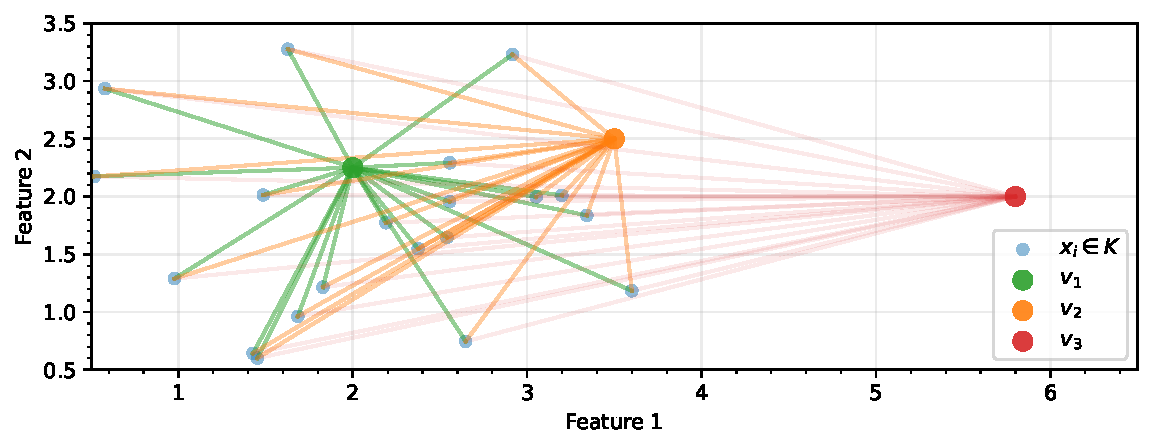
\includegraphics[width=\textwidth]{images/measures/abof-distance.pdf}
    \caption{Idea of the Angle-Based Outlier Factor applied as an outlierness measure.
             Element $v_1$ is located inside the cluster $T$,
             element $v_2$ is on the edge of the cluster $T$
             and element $v_3$ is a distant outlier;
             lines drawn correspond to vectors involved in the outlierness score calculation.}
    \label{fig:abof-idea}
\end{figure}

\begin{figure}[t]
    \centering
    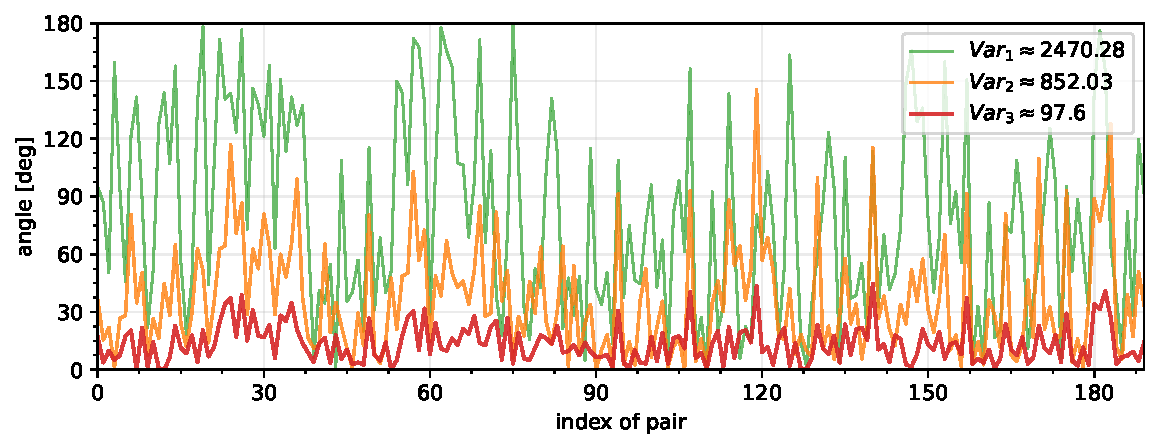
\includegraphics[width=\textwidth]{images/measures/abof-angles.pdf}
    \caption{Ranges of angles between vectors observed for various examined examples
             (typical point – $v_1$, edge point – $v_2$, outlier – $v_3$).
             For $20$ elements in cluster $T$, there are $190$ unique pairs in total,
             so $190$ angles possible for each of points $v_1$, $v_2$ and $v_3$.
             Highest variance is observed for an inlier, lowest variance in case of an outlier.}
    \label{fig:abof-angles}
\end{figure}

The Angle-Based Outlier Factor (ABOF/ABOD), proposed by Kriegel et al. \cite{Kriegel-2008}, is an anomaly detection technique that relies on the analysis of angles between feature vectors to determine whether the data is an outlier or not. Because of relying primarily on angles, instead of e.g., Euclidean distances, it is claimed to be effective even for applications in high-dimensional spaces.

Figure \ref{fig:abof-idea} illustrates the intuitive idea behind the algorithm. For any data point $v$ in the feature space $\mathbb{R}^d$ and a given data cluster $T$, there can be two vectors constructed between the point $v$ and points $x_1$, $x_2$ randomly selected from the cluster $T$. Then, the~angle $\alpha$ (or the value of $\cos(\alpha)$) between the constructed vectors may be calculated.

If the point $v$ is located within the data cluster $T$, then a wide spectrum of angles values may be observed, i.e., both acute and obtuse angles, as presented in figure \ref{fig:abof-angles}. Contrary, when the point $v$ is an outlier, a dominant number of acute angles with small variability of values shall be observed.

Mathematically this can be quantified by calculating the variance of angles values between the given data point $v$ and all possible pairs of points from the target cluster $T$. If the variance is high, i.e., a wide spectrum of angles is observed, the given data point is not an outlier. If the variance is low, the data point is likely to be an outlier.

Let $P$ be the set of all unique pairs $(x_1, x_2)$ – combinations of elements from the target cluster $T$. Then the outlierness score for a given vector $v$ can be calculated as
\begin{equation}
    ABOF(v, T) = \mathrm{Var}\left\{
        ~
        \forall (x_1, x_2) \in P:
        ~
        \frac{
            \vv{x_1 - v} ~\cdot~ \vv{x_2 - v}
        }{
            \norm{\vv{x_1 - v}}^2 \cdot \norm{\vv{x_2 - v}}^2
        }
        ~
    \right\}.
    \label{eq:abof}
\end{equation}

It shall be noticed that because all unique pairs from cluster $T$ are being considered, the computational complexity of the original algorithm is like $\mathcal{O}(n^3)$, hence for large datasets it rapidly becomes time ineffective. Therefore, even the original paper \cite{Kriegel-2008} additionally proposes variants of ABOF: approxABOF and LB-ABOF, that are faster to compute, based on various approximations, e.g., by subsampling the cluster $T$ to consider only $T$ nearest neighbors of point $v$, at the risk of lower accuracy.

In addition it can be observed that in equation \ref{eq:abof} the function formula is not based solely on the angular measure, because considering the scalar/dot product definition,
\begin{equation}
    \vv{v_1} \cdot \vv{v_2}
    =
    \norm{\vv{v_1}} \cdot \norm{\vv{v_2}} \cdot \cos(\alpha),
    \label{eq:dotproduct}
\end{equation}
the original formula \ref{eq:abof} may be therefore presented in a following alternative form,
\begin{equation}
    ABOF(v, T) = \mathrm{Var}\left\{
        ~
        \forall (x_1, x_2) \in P:
        ~
        \frac{
            \cos( \angle (\vv{x_1 - v}, \vv{x_2 - v}) )
        }{
            \norm{\vv{x_1 - v}} \cdot \norm{\vv{x_2 - v}}
        }
        ~
    \right\},
    \label{eq:abof-alt}
\end{equation}
where $\angle (\vv{x_1 - v}, \vv{x_2 - v})$ denotes the angle between vectors $\vv{x_1 - v}$ and $\vv{x_2 - v}$. This makes it visible that the original algorithm actually takes into account the angles that are normalized by the product of the length of the difference vectors \cite{Kriegel-2008}. When the analyzed point $v$ is far from the cluster $T$, the calculated angles are therefore contributing less to the outcome score value. Hence, literature \cite{Walkowiak-2018-asmbi} also discusses the purely angle-based variants without such additional scaling, that turns more accurate in some cases,
\begin{equation}
    ABOF2(v, T) = \mathrm{Var}\left\{
        ~
        \forall (x_1, x_2) \in P:
        ~
        \cos( \angle (\vv{x_1 - v}, \vv{x_2 - v}) )
        ~
    \right\}.
    \label{eq:abof2}
\end{equation}

During the research the own implementation (Section \ref{section:pyopenset}) was used, based on the description from the original article \cite{Kriegel-2008}. For convenience, the returned values were inverted, so the greater values indicate that data more likely to be outliers.
